\section{Modello di sviluppo}
Il modello di sviluppo adottato dal gruppo è il \textbf{modello incrementale}.
\subsection{Modello incrementale}
Il modello di sviluppo incrementale vede il progetto come una serie di rilasci (interni e/o esterni), cosicché ad ogni scadenza il materiale consegnato sia sempre più vicino al prodotto finale.
Questo approccio di sviluppo vede la specifica del software, la sua implementazione, convalida ed evoluzione come attività intrecciate tra loro e da sviluppare in parallelo. Quindi il prodotto è considerato tale solo all'ultimo rilascio. Motivo per cui si relaziona bene con il versionamento adottato per il sistema.
L'adozione dello sviluppo incrementale porta i seguenti vantaggi:
\begin{itemize}
\item costi ridotti di implementazione;
\item facilità nell'ottenere feedback;
\item possibilità di consegnare prototipi.
\end{itemize}
Svantaggi del modello incrementale:
\begin{itemize}
\item il processo non è visibile e il manager deve richiedere consegne frequenti e regolari;
\item inclinazione alla degradazione del sistema, ovvero la difficoltà di aggiungere funzionalità al sistema in un rilascio successivo, dopo averne integrata un'altra nella consegna attuale. Ad ogni incremento aumenta la complessità del codice e di conseguenza dei costi. È possibile rimediare tramite refactoring, anche se quest'ultimo muta il modello di sviluppo da incrementale a iterativo.
\end{itemize}
\begin{figure}[H]
	\centering
	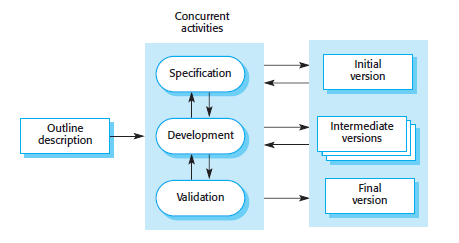
\includegraphics[width=0.70\linewidth]{img/incremental_development.png}
	\caption{Modello di sviluppo incrementale}
\end{figure}

\pagebreak
\subsubsection{Incrementi individuati}
Durante i periodi di Progettazione e Codifica per la Technology Baseline e Progettazione di Dettaglio sono stati individuati alcuni incrementi. \\
Di seguito verranno indicati tutti gli incrementi fatti con i relativi requisiti.


\begin{longtable}{C{4cm} L{3cm}}
\rowcolor{white}\caption{Tracciamento incrementi} \\
		\rowcolor{redafk}
\textcolor{white}{\textbf{Incremento}} &
\textcolor{white}{\textbf{Requisiti}} \\
		\endfirsthead
		\rowcolor{white}\caption[]{(continua)} \\
		\rowcolor{redafk}
\textcolor{white}{\textbf{Incremento}} &
\textcolor{white}{\textbf{Requisiti}} \\
		\endhead
Incremento 1: Ottenimento file JSON			& Re1F1 \newline Re1F.1  \newline Re1F1.2 \newline Re1F1.3 \newline Re1F1.4 \newline Re1F9\newline Re1F16 \\
Incremento 2: Caricamento file JSON			& Re1F2 \newline Re1F2.1 \newline Re1F2.2  \\
Incremento 3: Collegamento al flusso dati	& Re1F3.1 \newline Re1F3.2 \newline \\
\end{longtable}